% 若编译失败,且生成 .synctex(busy) 辅助文件,可能有两个原因:
% 1. 需要插入的图片不存在:Ctrl + F 搜索 'figure' 将这些代码注释/删除掉即可
% 2. 路径/文件名含中文或空格:更改路径/文件名即可

% --------------------- 文章宏包及相关设置 --------------------- %
% >> ------------------ 文章宏包及相关设置 ------------------ << %
% 设定文章类型与编码格式
    \documentclass[UTF8]{report}		

% 本 .tex 专属的宏定义
\def\V{\ \mathrm{V}}
\def\mV{\ \mathrm{mV}}
\def\kV{\ \mathrm{KV}}
\def\KV{\ \mathrm{KV}}
\def\MV{\ \mathrm{MV}}
\def\A{\ \mathrm{A}}
\def\mA{\ \mathrm{mA}}
\def\kA{\ \mathrm{KA}}
\def\KA{\ \mathrm{KA}}
\def\MA{\ \mathrm{MA}}
\def\O{\ \Omega}
\def\mO{\ \Omega}
\def\kO{\ \mathrm{K}\Omega}
\def\KO{\ \mathrm{K}\Omega}
\def\MO{\ \mathrm{M}\Omega}
\def\Hz{\ \mathrm{Hz}}

% 自定义宏定义
    \def\N{\mathbb{N}}
    \def\F{\mathbb{F}}
    \def\Z{\mathbb{Z}}
    \def\Q{\mathbb{Q}}
    \def\R{\mathbb{R}}
    \def\C{\mathbb{C}}
    \def\T{\mathbb{T}}
    \def\S{\mathbb{S}}
    \def\A{\mathbb{A}}
    \def\I{\mathscr{I}}
    \def\Im{\mathrm{Im\,}}
    \def\Re{\mathrm{Re\,}}
    \def\d{\mathrm{d}}
    \def\p{\partial}

% 导入基本宏包
    \usepackage[UTF8]{ctex}     % 设置文档为中文语言
    \usepackage[colorlinks, linkcolor=blue, anchorcolor=blue, citecolor=blue, urlcolor=blue]{hyperref}  % 宏包:自动生成超链接 (此宏包与标题中的数学环境冲突)
    % \usepackage{docmute}    % 宏包:子文件导入时自动去除导言区,用于主/子文件的写作方式,\include{./51单片机笔记}即可。注:启用此宏包会导致.tex文件capacity受限。
    \usepackage{amsmath}    % 宏包:数学公式
    \usepackage{mathrsfs}   % 宏包:提供更多数学符号
    \usepackage{amssymb}    % 宏包:提供更多数学符号
    \usepackage{pifont}     % 宏包:提供了特殊符号和字体
    \usepackage{extarrows}  % 宏包:更多箭头符号


% 文章页面margin设置
    \usepackage[a4paper]{geometry}
        \geometry{top=1in}
        \geometry{bottom=1in}
        \geometry{left=0.75in}
        \geometry{right=0.75in}   % 设置上下左右页边距
        \geometry{marginparwidth=1.75cm}    % 设置边注距离(注释、标记等)

% 配置数学环境
    \usepackage{amsthm} % 宏包:数学环境配置
    % theorem-line 环境自定义
        \newtheoremstyle{MyLineTheoremStyle}% <name>
            {11pt}% <space above>
            {11pt}% <space below>
            {}% <body font> 使用默认正文字体
            {}% <indent amount>
            {\bfseries}% <theorem head font> 设置标题项为加粗
            {:}% <punctuation after theorem head>
            {.5em}% <space after theorem head>
            {\textbf{#1}\thmnumber{#2}\ \ (\,\textbf{#3}\,)}% 设置标题内容顺序
        \theoremstyle{MyLineTheoremStyle} % 应用自定义的定理样式
        \newtheorem{LineTheorem}{Theorem.\,}
    % theorem-block 环境自定义
        \newtheoremstyle{MyBlockTheoremStyle}% <name>
            {11pt}% <space above>
            {11pt}% <space below>
            {}% <body font> 使用默认正文字体
            {}% <indent amount>
            {\bfseries}% <theorem head font> 设置标题项为加粗
            {:\\ \indent}% <punctuation after theorem head>
            {.5em}% <space after theorem head>
            {\textbf{#1}\thmnumber{#2}\ \ (\,\textbf{#3}\,)}% 设置标题内容顺序
        \theoremstyle{MyBlockTheoremStyle} % 应用自定义的定理样式
        \newtheorem{BlockTheorem}[LineTheorem]{Theorem.\,} % 使用 LineTheorem 的计数器
    % definition 环境自定义
        \newtheoremstyle{MySubsubsectionStyle}% <name>
            {11pt}% <space above>
            {11pt}% <space below>
            {}% <body font> 使用默认正文字体
            {}% <indent amount>
            {\bfseries}% <theorem head font> 设置标题项为加粗
            {:\\ \indent}% <punctuation after theorem head>
            {0pt}% <space after theorem head>
            {\textbf{#3}}% 设置标题内容顺序
        \theoremstyle{MySubsubsectionStyle} % 应用自定义的定理样式
        \newtheorem{definition}{}

%宏包:有色文本框(proof环境)及其设置
    \usepackage[dvipsnames,svgnames]{xcolor}    %设置插入的文本框颜色
    \usepackage[strict]{changepage}     % 提供一个 adjustwidth 环境
    \usepackage{framed}     % 实现方框效果
        \definecolor{graybox_color}{rgb}{0.95,0.95,0.96} % 文本框颜色。修改此行中的 rgb 数值即可改变方框纹颜色,具体颜色的rgb数值可以在网站https://colordrop.io/ 中获得。(截止目前的尝试还没有成功过,感觉单位不一样)(找到喜欢的颜色,点击下方的小眼睛,找到rgb值,复制修改即可)
        \newenvironment{graybox}{%
        \def\FrameCommand{%
        \hspace{1pt}%
        {\color{gray}\small \vrule width 2pt}%
        {\color{graybox_color}\vrule width 4pt}%
        \colorbox{graybox_color}%
        }%
        \MakeFramed{\advance\hsize-\width\FrameRestore}%
        \noindent\hspace{-4.55pt}% disable indenting first paragraph
        \begin{adjustwidth}{}{7pt}%
        \vspace{2pt}\vspace{2pt}%
        }
        {%
        \vspace{2pt}\end{adjustwidth}\endMakeFramed%
        }

% 外源代码插入设置
    % matlab 代码插入设置
    \usepackage{matlab-prettifier}
        \lstset{
            style=Matlab-editor,  % 继承matlab代码颜色等
        }
    \usepackage[most]{tcolorbox} % 引入tcolorbox包 
    \usepackage{listings} % 引入listings包
        \tcbuselibrary{listings, skins, breakable}
        \lstdefinestyle{matlabstyle}{
            language=Matlab,
            basicstyle=\small,
            breakatwhitespace=false,
            breaklines=true,
            captionpos=b,
            keepspaces=true,
            numbers=left,
            numbersep=15pt,
            showspaces=false,
            showstringspaces=false,
            showtabs=false,
            tabsize=2
        }
        \newtcblisting{matlablisting}{
            arc=0pt,
            top=0pt,
            bottom=0pt,
            left=1mm,
            listing only,
            listing style=matlabstyle,
            breakable,
            colback=white   % 选一个合适的颜色
        }

% table 支持
    \usepackage{booktabs}   % 宏包:三线表
    \usepackage{tabularray} % 宏包:表格排版
    \usepackage[longtable]{multirow} % 宏包:multi 行列
    \usepackage{longtable}  % 宏包:长表格

% figure 设置
    \usepackage{graphicx}  % 支持 jpg, png, eps, pdf 图片 
    \usepackage{svg}       % 支持 svg 图片
        \svgsetup{
            % 指向 inkscape.exe 的路径
            inkscapeexe = D:/aa_my_apps_main/Inkscape/bin/inkscape.exe, 
            % 一定程度上修复导入后图片文字溢出几何图形的问题
            inkscapelatex = false                 
        }
    \usepackage{subcaption} % 支持子图

% 图表进阶设置
    \usepackage{caption}    % 图注、表注
        \captionsetup[figure]{name=图}  
        \captionsetup[table]{name=表}
        \captionsetup{labelfont=bf, font=small}
    \usepackage{float}     % 图表位置浮动设置 

% 圆圈序号自定义
    \newcommand*\circled[1]{\tikz[baseline=(char.base)]{\node[shape=circle,draw,inner sep=0.8pt, line width = 0.03em] (char) {\small \bfseries #1};}}   % TikZ solution

% 列表设置
\usepackage{enumitem}   % 宏包:列表环境设置
    \setlist[enumerate]{itemsep=0pt, parsep=0pt, topsep=0pt, partopsep=0pt, leftmargin=3.5em} 
    \setlist[itemize]{itemsep=0pt, parsep=0pt, topsep=0pt, partopsep=0pt, leftmargin=3.5em}
    \newlist{circledenum}{enumerate}{1} % 创建一个新的枚举环境  
    \setlist[circledenum,1]{  
        label=\protect\circled{\arabic*}, % 使用 \arabic* 来获取当前枚举计数器的值,并用 \circled 包装它  
        ref=\arabic*, % 如果需要引用列表项,这将决定引用格式(这里仍然使用数字)
        itemsep=0pt, parsep=0pt, topsep=0pt, partopsep=0pt, leftmargin=3.5em
    }  
    

% 文章默认字体设置
\usepackage{fontspec}   % 宏包:字体设置
    \setmainfont{SimSun}    % 设置中文字体为宋体字体
    \setmainfont{Times New Roman} % 设置英文字体为Times New Roman

% 文章序言设置
    \newcommand{\cnabstractname}{序言}
    \newenvironment{cnabstract}{%
        \par\Large
        \noindent\mbox{}\hfill{\bfseries \cnabstractname}\hfill\mbox{}\par
        \vskip 2.5ex
        }{\par\vskip 2.5ex}

% 参考文献引用设置
    \bibliographystyle{unsrt}   % 设置参考文献引用格式为unsrt
    \newcommand{\upcite}[1]{\textsuperscript{\cite{#1}}}     % 自定义上角标式引用

% 各级标题自定义设置
    \usepackage{titlesec}   
    % chapter
        \titleformat{\chapter}[hang]{\normalfont\Large\bfseries\centering}{Homework \thechapter :}{10pt}{}
        \titlespacing*{\chapter}{0pt}{-30pt}{10pt} % 控制上方空白的大小
    % section
        \titleformat{\section}[hang]{\normalfont\large\bfseries}{\thesection}{8pt}{}
    % subsection
        %\titleformat{\subsubsection}[hang]{\normalfont\bfseries}{}{8pt}{}
    % subsubsection
        %\titleformat{\subsubsection}[hang]{\normalfont\bfseries}{}{8pt}{}

% --------------------- 文章宏包及相关设置 --------------------- %
% >> ------------------ 文章宏包及相关设置 ------------------ << %



% ------------------------ 文章信息区 ------------------------ %
% >> --------------------- 文章信息区 --------------------- << %
% 页眉页脚设置
\usepackage{fancyhdr}   %宏包:页眉页脚设置
    \pagestyle{fancy}
    \fancyhf{}
    \cfoot{\thepage}
    \renewcommand\headrulewidth{1pt}
    \renewcommand\footrulewidth{0pt}
    \chead{电路原理作业,\ 丁毅,\ 2023K8009908031}
    \lhead{Homework \thechapter}
    \rhead{dingyi233@mails.ucas.ac.cn}

%文档信息设置
\title{电路原理课程作业\\ Homework of Principles of Electric Circuits }
\author{丁毅\\ \footnotesize 中国科学院大学,北京 100049\\ Yi Ding \\ \footnotesize University of Chinese Academy of Sciences, Beijing 100049, China}
\date{\footnotesize 2024.8 -- 2025.1}
% >> --------------------- 文章信息区 --------------------- << %
% ------------------------ 文章信息区 ------------------------ %

% 开始编辑文章

\begin{document}
\zihao{5}           % 设置全文字号大小

% ------------------------ 封面序言与目录 ------------------------ %
% >> --------------------- 封面序言与目录 --------------------- << %
% 封面
    \maketitle\newpage  
    \pagenumbering{Roman} % 页码为大写罗马数字
    \thispagestyle{fancy}   % 显示页码、页眉等

% 序言
    \begin{cnabstract}\normalsize 
        本文为笔者本科时的“电路原理”课程作业(Homework of Principles of Electric Circuits, 2024.9-2025.1)。由于个人学识浅陋,认识有限,文中难免有不妥甚至错误之处,望读者不吝指正,在此感谢。\par 
        我的邮箱是 dingyi233@mails.ucas.ac.cn。
    \end{cnabstract}
    \addcontentsline{toc}{chapter}{序言} % 手动添加为目录

% 不换页目录
    \setcounter{tocdepth}{0}
    \noindent\rule{\textwidth}{0.1em}   % 分割线
    \noindent\begin{minipage}{\textwidth}\centering 
        \vspace{1cm}
        \tableofcontents\thispagestyle{fancy}   % 显示页码、页眉等   
    \end{minipage}  
    \addcontentsline{toc}{chapter}{目录} % 手动添加为目录

% 收尾工作
    \newpage    
    \pagenumbering{arabic} 

% >> --------------------- 封面序言与目录 --------------------- << %
% ------------------------ 封面序言与目录 ------------------------ %

\chapter{2024.8.27 - 2024.9.2}\thispagestyle{fancy}

\section{习题集 1-2}

\begin{enumerate}
\item[(a)] 短路,因此 $U = 0,\  I = \frac{U_S}{R_i}$
\item[(b)] 开路,因此 $U = U_s, \ I = 0$
\item[(c)] 构成回路,因此  $ U = \frac{U_SR}{R + R_i},\ I = \frac{U_S}{R + R_i}$ 
\end{enumerate}

\begin{figure}[H]\centering
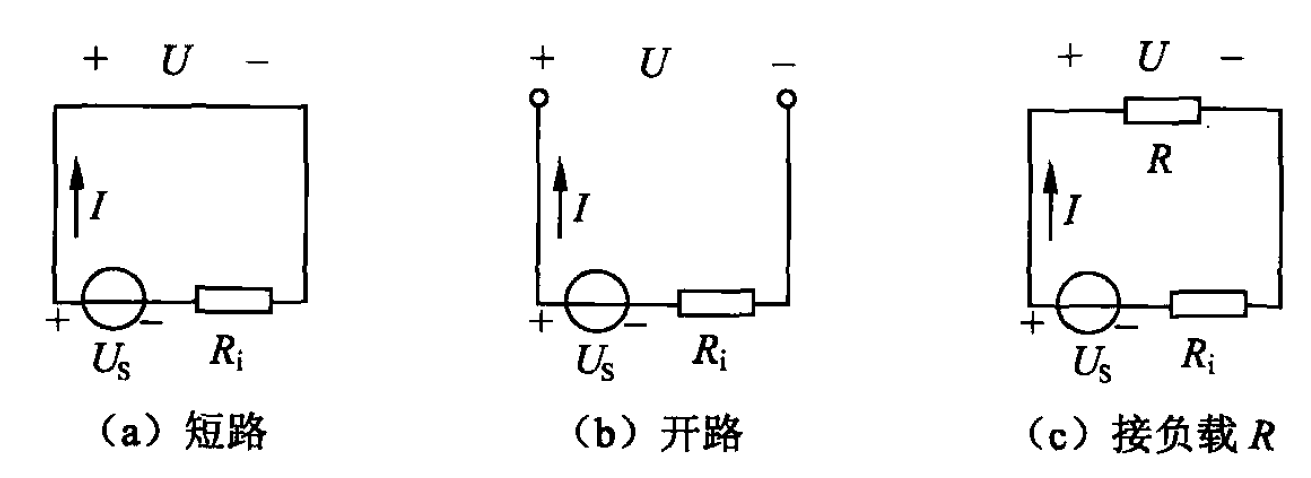
\includegraphics[width=0.6\textwidth]{assets/1/ae1cfc03fad5c98bfff08a663714a004.png}
\end{figure}

\section{习题集 1-9}

\begin{enumerate}
    \item[(a)]  $ \varphi_a - 3\ \mathrm{V} + 2\ \mathrm{V} = \varphi_b \Longrightarrow U_{ab} = 1\ \mathrm{V} $ 
    \item[(b)] $I = 1\ \mathrm{A},\  3 -IR= -4 \Longrightarrow R = 7\ \Omega$ 
    \item[(c)] $-3 + U_S = 1 \Longrightarrow U_S = 4 \ \mathrm{V}$ 
    \item[(d)] $R=2\ \Omega,\ -IR + 2 = 3 \Longrightarrow I = -0.5\ \mathrm{A}$ 
\end{enumerate}

\begin{figure}[H]\centering
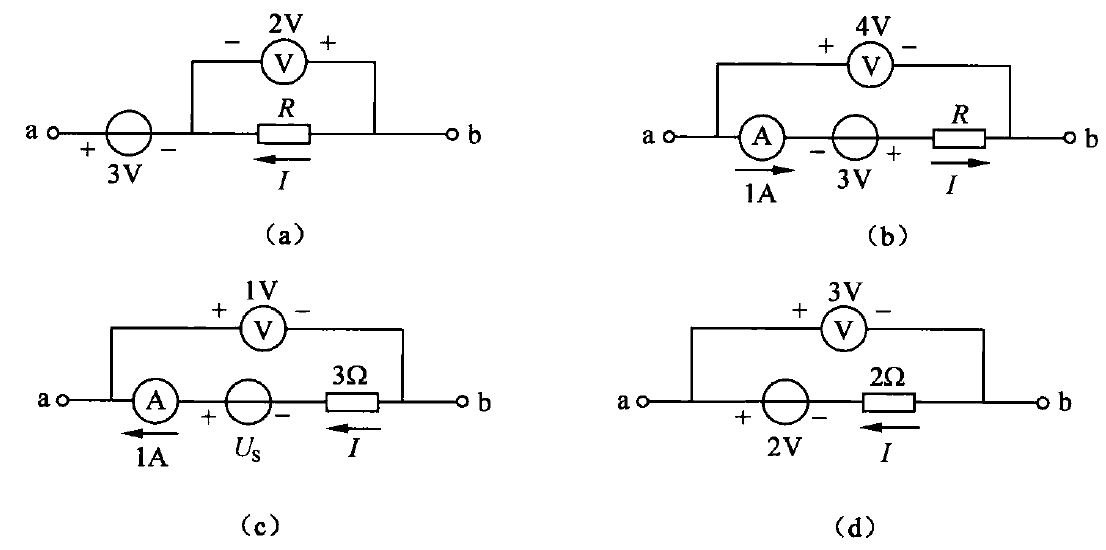
\includegraphics[width=0.6\textwidth]{assets/1/d3d69ecd6b1c1bc476fd4a4957fb9e56.png}
\end{figure}

\section{习题集 1-10}



\begin{enumerate}
\item[(a)] 
记参考点 a 的电势 $\varphi_a=0$,则 $\varphi_c = 2\ \mathrm{V} ,\ \varphi_b = -2\ \mathrm{V}$,因此 $U_{ab} = 2\ \mathrm{V}$

\item[(b)] 
记参考点 d 的电势 $\varphi_d = \varphi_b =0$,则 $\varphi_c = 6\ \mathrm{V},\ \varphi_a = -2\ \mathrm{V}$,因此 $U_{ab} = -2\ \mathrm{V}$

\end{enumerate}

\begin{figure}[H]\centering
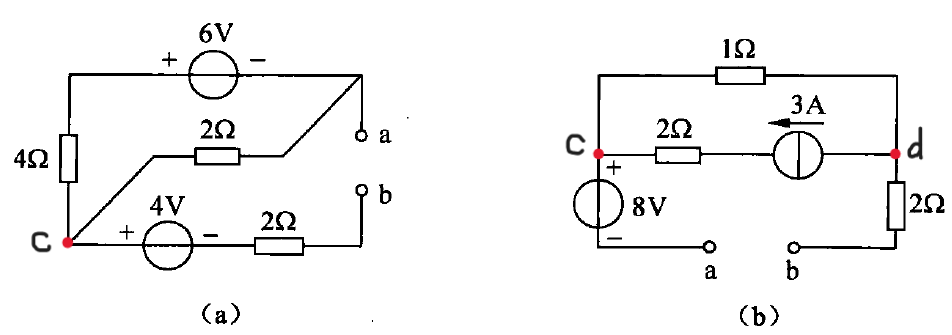
\includegraphics[width=0.55\textwidth]{assets/1/9dda9e5f333b8cb7f498d15c015e5fd0.png}
\end{figure}
{\par\color{gray}\small
后补:(b) 中电流源两端仍有电势差,$\varphi_c \ne 6 \ \mathrm{V}$ 而是 $ \varphi_c = -3\ \mathrm{V} $,最终得 $U_{ab} = -5 \ \mathrm{V}$。
\par}


\section{习题集 1-15}

\begin{enumerate}
    \item[(a)] $I = -\frac{U}{R} + 4\ \mathrm{A} = -2 \ \mathrm{A}$
    \item[(b)] $U =12 \ \mathrm{V} + 3\ \Omega \times 4 \ \mathrm{A} = 0 $ 
    \item[(c)] $I = 8 \ \mathrm{A} - 6\ \mathrm{A} = 2 \ \mathrm{A}$,$ U = 12 \ \mathrm{V} + 3\times8 \ \mathrm{V} = 36 \ \mathrm{V}$ 
    \item[(d)] 取点 $ d $ 为参考点,则 $\varphi_d = \varphi_c = 0$,$\varphi_b = \varphi_a = 9 \ \mathrm{V}$,于是 $U_1 = 9 + 2\times3 = 15\ \mathrm{V},\ U_2 = 9 + 2\times 2 = 13 \ \mathrm{V},\ I =2 -  (9-3) = - 4 \ \mathrm{A}$
\end{enumerate}

\begin{figure}[H]\centering
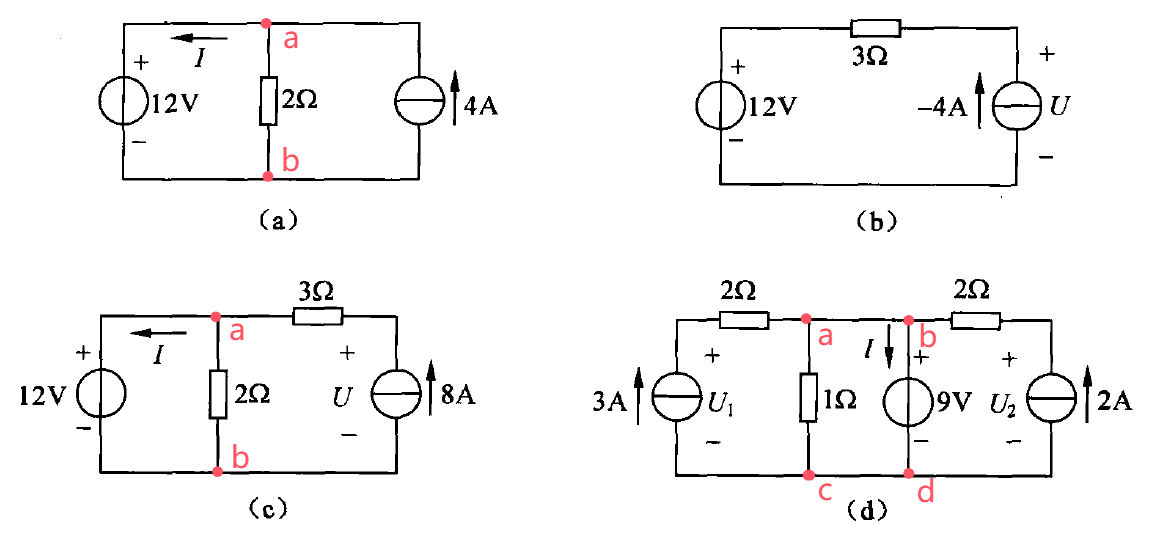
\includegraphics[width=0.7\textwidth]{assets/1/b82ef4f3b4efd9d0ee903e5f19353345.png}
\end{figure}

\section{习题集 1-29}

取点 $a$ 为参考点 $\varphi_a = 0$,可得 $\varphi_b = 100U_1 - 80$,于是在结点 $a$ 有电流:
\begin{equation*}
I_S + \frac{100U_1 - 80}{5} = 2
\end{equation*}

$0.2\ \Omega$ 电阻处又有 $U_1 = 0.2 I_S$,联立解得 $I_S = 3.6 \ \mathrm{A}, U_1 = 7.2 \ \mathrm{V}$。

\section{习题集 1-30}

这里要注意左二元器件是受控电流源,因此 $0.5U$ 是指电流大小而非电压。$I_1$ 处可列出方程:

\begin{equation*}
\frac{U}{2} + 12 - \frac{U}{3} = 0.5U \Longrightarrow U = 36 \ \mathrm{V} \Longrightarrow P = UI = 432 \ \mathrm{W}
\end{equation*}

\begin{figure}[H]\centering
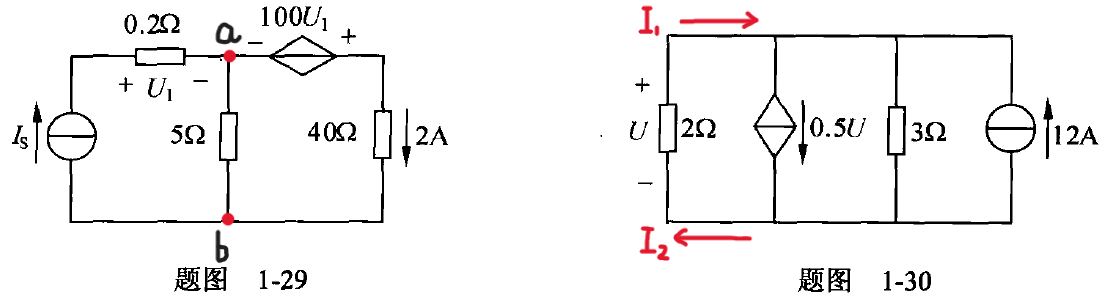
\includegraphics[width=0.7\textwidth]{assets/1/94b342032a5f6622a60b3c9d99e37993.png}
\end{figure}

{\par\color{gray}\small
后补:上面的方程列错了,错将 $I_1$ 的方向标为由左向右,应该是由右向左。最后得到 $P = 108\ \mathrm{W}$。另外,也可以直接将受控电流源看作是 2 $\Omega$ 的电阻,这样左侧三个电阻并联,也可求出正确答案 108 W.
\par}


\section{讲义题 1-6}

$\alpha > 90 \text{\textdegree}$ 时,电阻为“负电阻”。

\section{讲义题 1-7}


\begin{definition}[充放电倍率 C 的含义]
C (充放电倍率)表示电池充放电时电流相对电池容量的大小数值,$\mathrm{C} = \frac{\text{电池容量}}{\text{充放电所需时间}}$。例如,1 C 电流充电表示电池需要 1 小时充满,5 C 充电表示电池需要 $0.2$ 小时充满。放电也是类似的,一个 10 Ah 的电池以 2 C 放电,表示以 20 A 的电流放电 0.5 h。 \par
若倍率上升,总时间就会下降,若倍率下降,总时间就会上升。通俗来讲,$C$ 代表了电池的爆发力大小,高倍率的动力电池瞬间放电电流大,特别适合大电流放电产品使用,如航模。
\end{definition}


\begin{definition}[涓流充电]
涓流充电是指在电池接近完全充满电后,采用非常小的电流进行充电,以弥补电池自放电造成的容量损失。理论倍率 C 约为 最大倍率 $\mathrm{C_{max}}$ 的 $\frac{1}{100}$ 至 $\frac{1}{1000}$,但由于倍率太小,常常根本无法充电,一个比较好的方法是脉冲式充电,例如以 $\frac{\mathrm{C_{max}}}{10}$ 充电 6 s,然后停止充电 54 s。
\end{definition}


\begin{definition}[快速充电]
快速充电至少要求 1 C,现阶段的快速充电多在 1.5 C 至 2 C 之间。
\end{definition}


\section{讲义题 1-8(Multisim 仿真)}

仿真电路如图 \ref{仿真电路图} 所示,

\begin{figure}[H]\centering
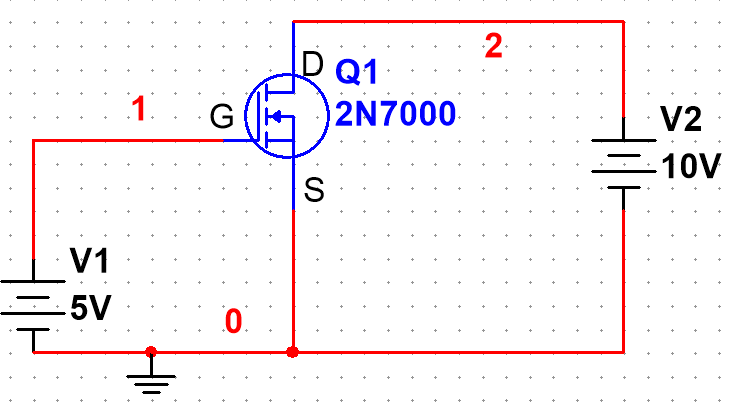
\includegraphics[width=0.36\textwidth]{assets/1/5c45ed5b5258df3fa8e1babac4a7ace2.png}
\caption{\textbf{仿真电路图}}\label{仿真电路图}
\end{figure}

先固定 $U_{GS} = 5\ \mathrm{V}$ 不变(即 $V_1 = 5\ \mathrm{V}$),横坐标 $U_{DS} \in [0\ \mathrm{V},\ 12\ \mathrm{V}]$,画出 $I_{DS}$(即 $I_2$)的变化曲线,如图 \ref{仿真结果1} 所示。再固定 $U_{DS} = 10\ \mathrm{V}$ 不变(即 $V_2 = 10\ \mathrm{V}$),横坐标 $U_{GS} \in [0\ \mathrm{V},\ 10\ \mathrm{V}]$,画出 $I_{DS}$(即 $I_2$)的变化曲线,如图 \ref{仿真结果2} 所示。
\begin{center}
    \noindent\begin{minipage}{0.42\textwidth}
        \begin{figure}[H]\centering
        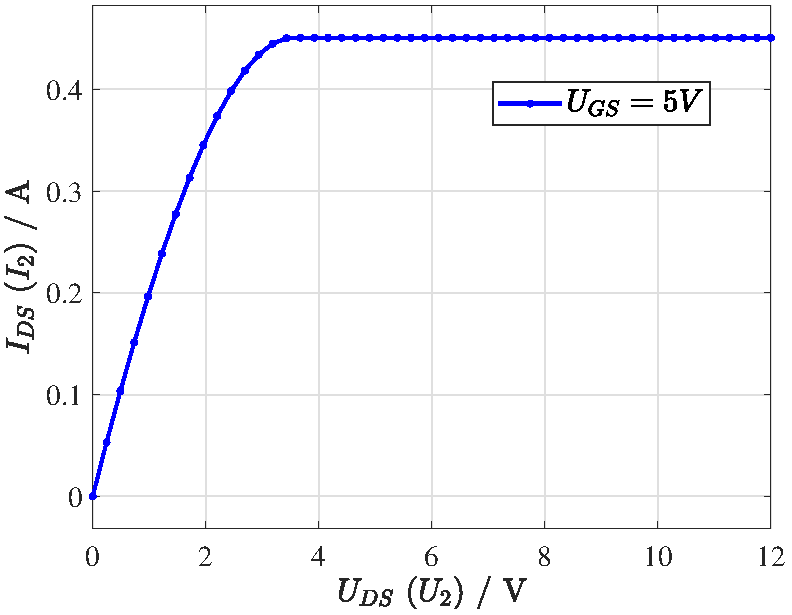
\includegraphics[width=\textwidth]{assets/1/2024-08-30_00-57-32.pdf}
        \caption{\textbf{仿真结果1}}\label{仿真结果1}
        \end{figure}
    \end{minipage}\hspace{5mm}
    \begin{minipage}{0.42\textwidth}
        \begin{figure}[H]\centering
        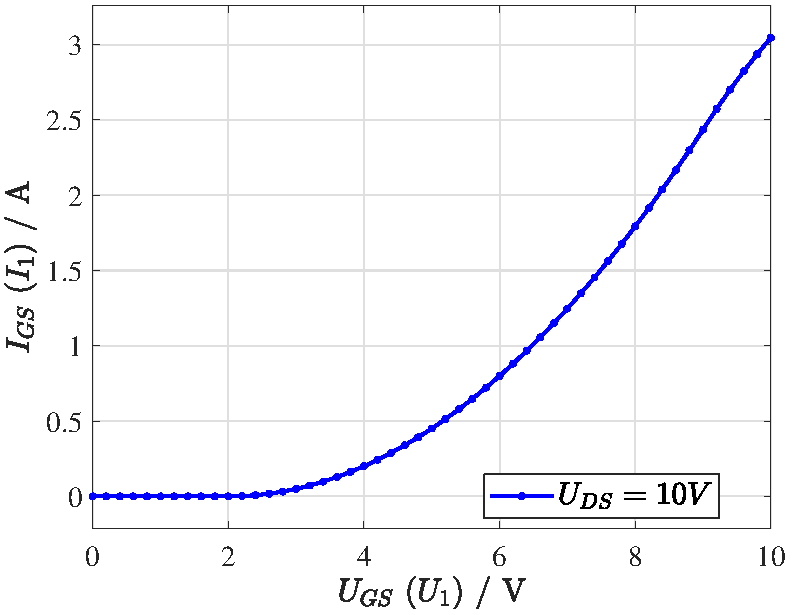
\includegraphics[width=\textwidth]{assets/1/2024-08-30_00-57-34.pdf}
    \caption{\textbf{仿真结果2}}\label{仿真结果2}
    \end{figure}
    \end{minipage}
\end{center}


\chapter{2024.9.3 - 2024.9.9}\thispagestyle{fancy}

\section{习题集 1-33}
左半边回路有:
\begin{gather*}
u_1 - 67i_e - (1-\alpha)i_e \cdot 150 = 0 \Longrightarrow \frac{u_2}{u_1} = \frac{\alpha i_eR_L }{70i_e} = \frac{0.98\times 1500}{70} = 21 \\ 
p_2 = (\alpha i_e)^2R_L, \quad p_1 = u_1 i_e \Longrightarrow \frac{p_2}{p_1} = \frac{(\alpha i_e)^2R_L}{70i_e^2} = 20.58
\end{gather*}

\begin{figure}[H]\centering
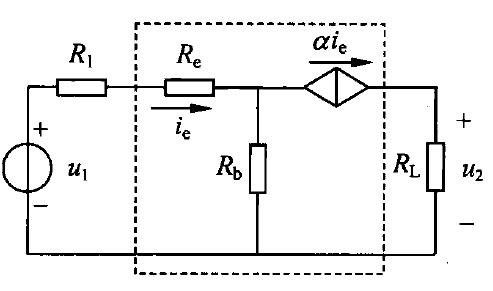
\includegraphics[width=0.5\textwidth]{assets/2/image (47).jpg}
\caption{\textbf{习题集 1-33}}
\end{figure}


\section{习题集 2-2}
对图 (a),化简并联后电桥平衡,可以得到
\begin{equation*}
\frac{1}{R} = \frac{1}{20 } + \frac{1}{40} +\frac{1}{40} \Longrightarrow R = 10\ \Omega
\end{equation*}
对图 (b),经过多次并联化简,可以得到:
\begin{equation}
R = 8 + \frac{3\times 6}{3+6}=10\ \Omega
\end{equation}
\begin{figure}[H]\centering
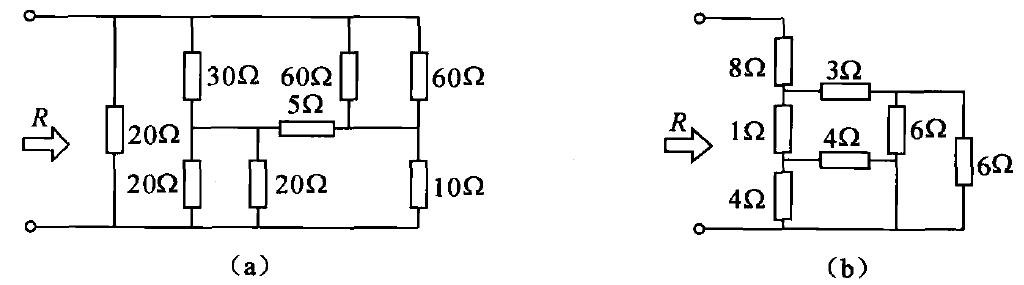
\includegraphics[width=0.85\textwidth]{assets/2/e02c39d3f229a4b6352b828e57c3737f.jpg}
\caption{\textbf{习题集 2-2}}
\end{figure}

\section{习题集 2-6}

各电路的最简电路图如图 \ref{习题集 2-6 解答} 所示: 

\noindent\begin{minipage}{0.50\textwidth}
    \begin{figure}[H]\centering
        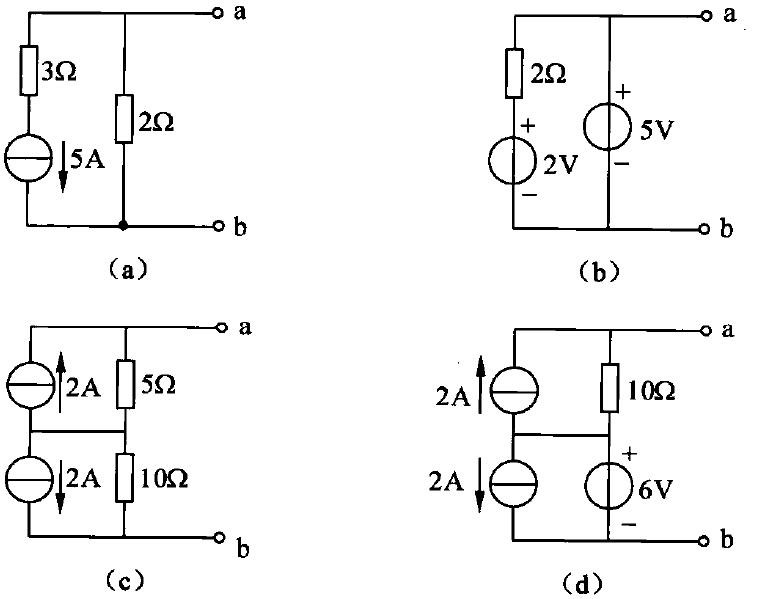
\includegraphics[height=190pt]{assets/2/bfc7d58924b9eaf9582656c984bd2c3b.jpg}
        \caption{\textbf{习题集 2-6}}
    \end{figure}
\end{minipage}\hfill
\begin{minipage}{0.50\textwidth}
    \begin{figure}[H]\centering
        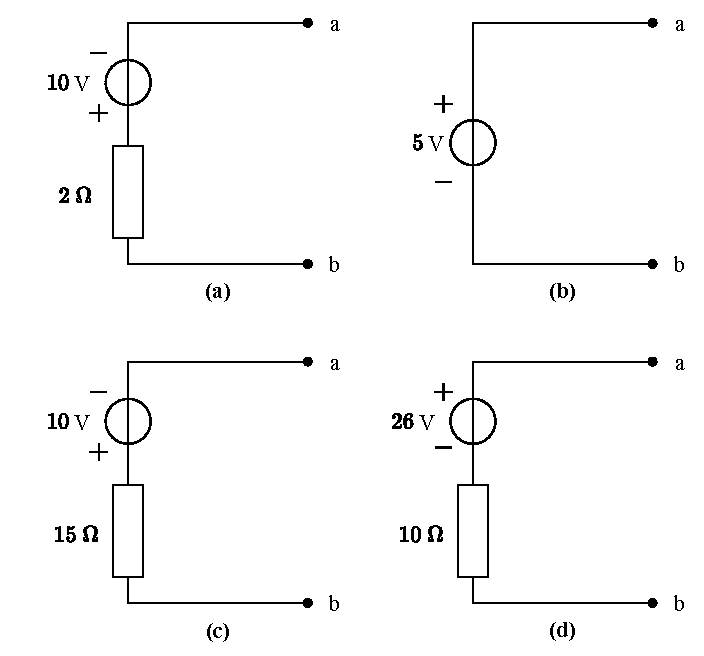
\includegraphics[height=190pt]{assets/2/2-6.drawio.pdf}
        \caption{\textbf{习题集 2-6 解答}}\label{习题集 2-6 解答}
    \end{figure}        
\end{minipage}


\section{习题集 2-8}

对原电路进行多次等效转换,得到最简电路如图所示,进而有:
\begin{equation*}
I = \frac{3}{2+3+5} = 0.3\ \mathrm{A}
\end{equation*}

\noindent\begin{minipage}{0.49\textwidth}
    \begin{figure}[H]\centering
        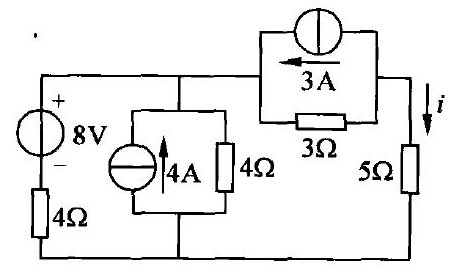
\includegraphics[height=120pt]{assets/2/78abd22edee32bbd38134d510246a9ab.jpg}
        \caption{\textbf{习题集 2-8}}
    \end{figure}
\end{minipage}\hfill
\begin{minipage}{0.49\textwidth}
\begin{figure}[H]\centering
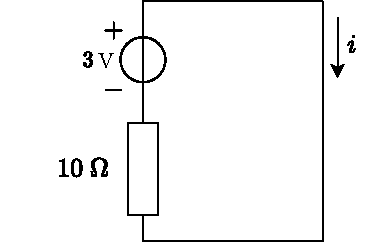
\includegraphics[height=120pt]{assets/2/2-8.drawio.pdf}
\caption{\textbf{习题集 2-8 等效电路}}\label{习题集 2-8 等效电路}
\end{figure}
\end{minipage}

\section{习题集 2-11}

等效电路图如图 \ref{习题集 2-11 等效电路} 所示,由 KVL 得:
\begin{gather*}
28 = 4I' + 4(I' - I),\quad 25 = -8I + 4(I' - I) \Longrightarrow I' = 2.95\ \mathrm{A},\ I = -1.1\ \mathrm{A}
\end{gather*}


\noindent\begin{minipage}{0.55\textwidth}
\begin{figure}[H]\centering
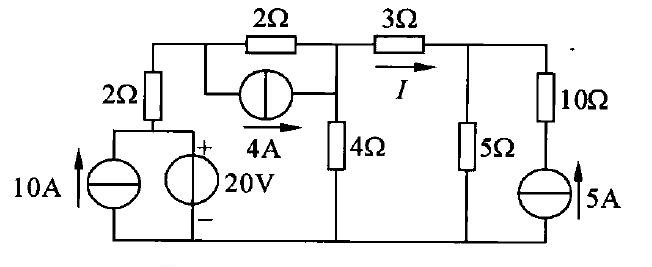
\includegraphics[height=110pt]{assets/2/1187c3e12fa1e6bd8d2019d53bd2752a.jpg}
\caption{\textbf{习题集 2-11}}
\end{figure}
\end{minipage}\hfill
\begin{minipage}{0.43\textwidth}
\begin{figure}[H]\centering
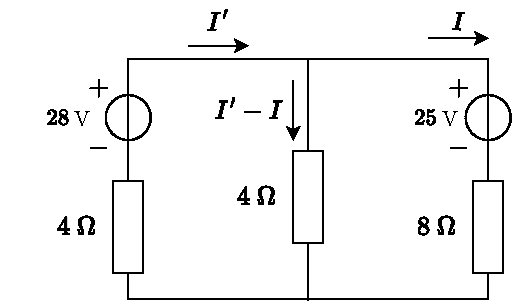
\includegraphics[height=110pt]{assets/2/2-11.drawio.pdf}
\caption{\textbf{习题集 2-11 等效电路}}\label{习题集 2-11 等效电路}
\end{figure}
\end{minipage}

\section{习题集 2-17}

等效电路图如图 \ref{2-17} 所示,可以求得:
\begin{equation*}
4I - 8 = 12(I-1) \Longrightarrow I = 0.5\ \mathrm{A}\Longrightarrow U = 8 - 8I = 4\ \mathrm{V}
\end{equation*}


\noindent\begin{minipage}{0.49\textwidth}
\begin{figure}[H]\centering
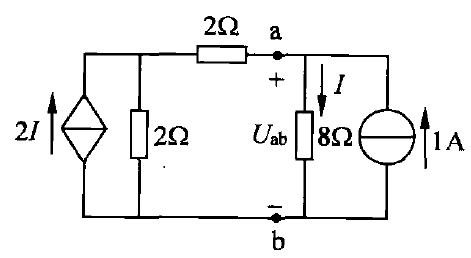
\includegraphics[height=120pt]{assets/2/78473b1c403974e048249bbdbf6a152f.jpg}
\caption{\textbf{习题集 2-17}}
\end{figure}
\end{minipage}\hfill
\begin{minipage}{0.49\textwidth}
\begin{figure}[H]\centering
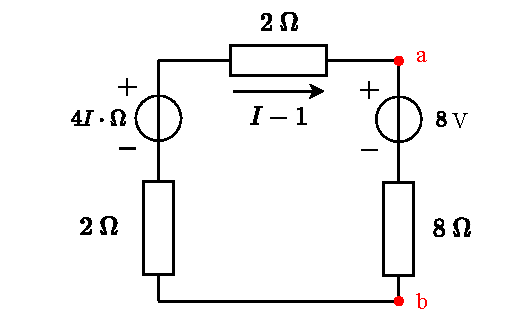
\includegraphics[height=120pt]{assets/2/2-17.drawio.pdf}
\caption{\textbf{习题集 2-17 等效电路}}\label{2-17}
\end{figure}
\end{minipage}



\section{习题集 2-22}

经过电源等效和 $\Delta$-Y 变换,等效电路图如图 \ref{2-22} 所示,回路总电阻 $R = 3 + \frac{4}{9} + \frac{14}{9} = 5\ \Omega$,\ $I_1 = \frac{U}{R} = 1.2\ \mathrm{A}$,则有:
\begin{equation*}
U_1 = 6 - 3\times 1.2 = 2.4\ \mathrm{V},\ U_2 = 2\times \frac{I}{2} = 1.2\ \mathrm{V},\quad P = 2 U_1 = 4.8\ \mathrm{W}
\end{equation*}

\noindent\begin{minipage}{0.49\textwidth}
\begin{figure}[H]\centering
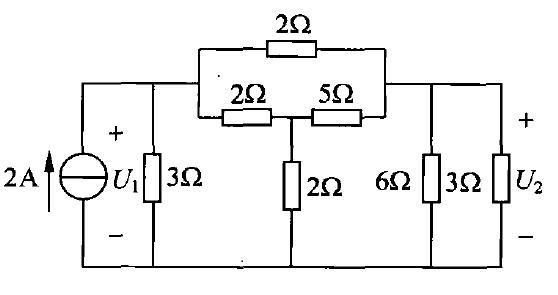
\includegraphics[height=110pt]{assets/2/0c8d1f0fb90ef6983c0aef6451919e4b.jpg}
\caption{\textbf{习题集 2-22}}
\end{figure}
\end{minipage}\hfill
\begin{minipage}{0.49\textwidth}
\begin{figure}[H]\centering
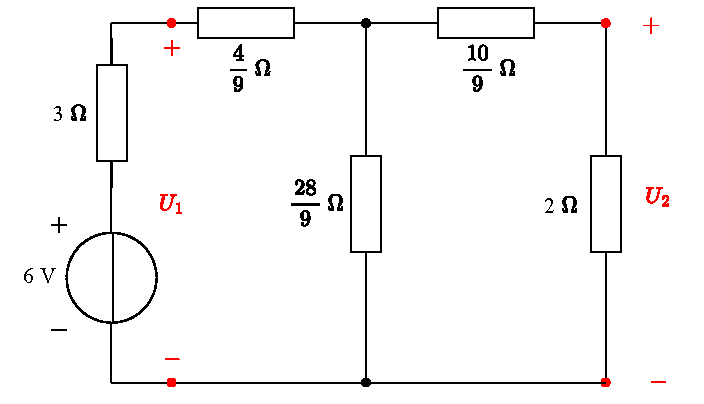
\includegraphics[height=110pt]{assets/2/2-22.drawio.pdf}
\caption{\textbf{习题集 2-22}}\label{2-22}
\end{figure}
\end{minipage}

\newpage
\section{\color[rgb]{0.2,0.9,0.2}(非作业) 习题集 2-4 (b)}
\section{\color[rgb]{0.2,0.9,0.2}(非作业) 习题集 2-5}
\section{\color[rgb]{0.2,0.9,0.2}(非作业) 习题集 2-5}














\chapter{2024.9.10 - 2024.9.16}\thispagestyle{fancy}


\section{习题集 3-40(书上答案不正确)}

由虚短和虚断,可以得到 $R_1$ 处电流为 $i_1 = \frac{u_s}{R_1}$(从上至下),于是输出电压 $u_o = 3u_s$,右侧负载由三个电阻构成,并联电阻分压 $2u_s$,最后得电流 $i(t)$:
\begin{equation}
i(t) = \frac{2u_s}{6 \KO} = \frac{u_s}{3} \mA
\end{equation}

\begin{figure}[H]\centering
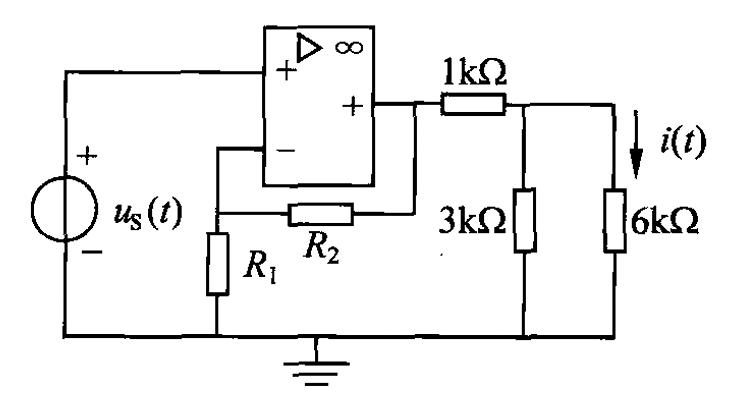
\includegraphics[width=0.4\textwidth]{assets/3/3-40.jpg}
\caption{\bfseries 习题集 3-40}
\end{figure}

\section{习题集 3-45(注意题目单位是 S)}

如图所示,将电导全部转换为电阻。由虚断、虚短,流经 $\frac{1}{10}\ \Omega$ 电阻的电流为 $i_1 = \frac{u_s}{0.1\ \Omega} = 10u_s$。右下角两电阻分压,再由虚短可得 $i_2 = 2U_o$,于是 $i_3 = i_1 + i_2 = 10 U_s + 2U_o$,由 KVL:
\begin{equation}
0 - \frac{1}{3}(10 U_s + 2U_o) = U_o \Longrightarrow  \frac{U_o}{U_s} = -2
\end{equation}
入端电阻 $R_i$: 
\begin{equation}
    i_1 = 10U_s \Longrightarrow  R_i = \frac{1}{10}\ \Omega
\end{equation}

\section{习题集 3-46}

依据 KVL、KCL、虚短、虚断,标出各节点电势,如图所示。则有:
\begin{equation}
(u_i+u_o)-u_o = i_LR,\ i_L = \frac{u_o}{R_L} \Longrightarrow u_o = u_i,\ i_L = \frac{u_o}{R_L} = \frac{u_i}{R_L}
\end{equation}

\begin{figure}[H]\centering
    \begin{subfigure}[t]{0.43\textwidth}\centering
        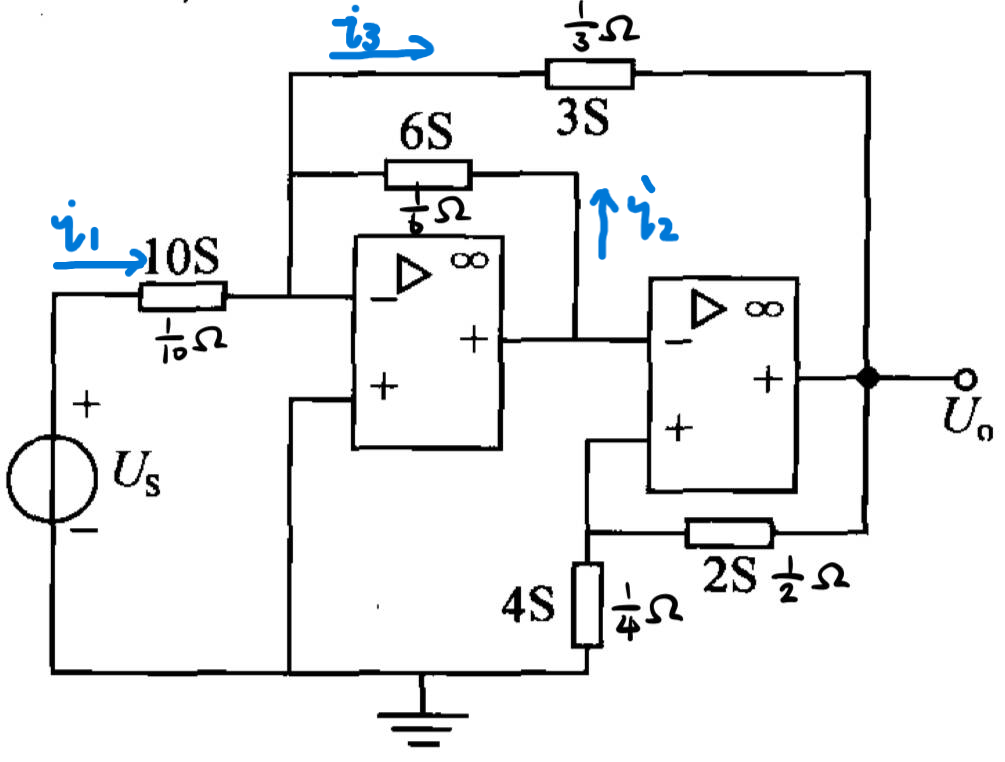
\includegraphics[height=150pt]{assets/3/3-45.png}
        \caption{\bfseries 习题集 3-45 }
    \end{subfigure}\begin{subfigure}[t]{0.43\textwidth}\centering
        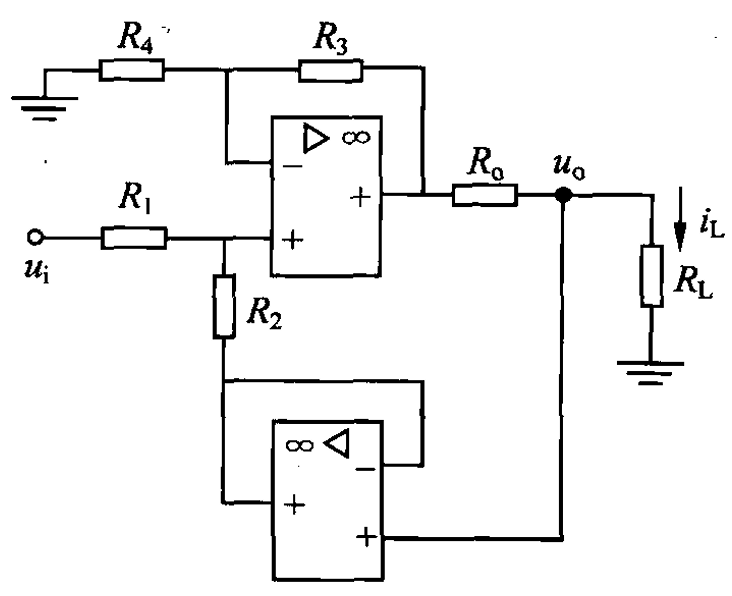
\includegraphics[height=150pt]{assets/3/3-46.png}
        \caption{\bfseries 习题集 3-46 }
    \end{subfigure}
    \caption{\bfseries 习题集 3-45 和习题集 3-46 }
    \end{figure}
    


\section{讲义题 2-19}
\textbf{(1)\ 反相比例放大器}

对输入电阻,$i_1 = \frac{u_i}{R_1} \Longrightarrow R_i = R_1$。对输出电阻,将输入电压源短路,采用加流求压法,在输出端接入电流源,由 $u = iR$ 且 $u=0$,得 $R_o = 0$。也即:
\begin{equation}
R_i = R_1,\ R_o = 0
\end{equation}

\textbf{(2)\ 同相比例放大器}

对输入电阻,$R_1$ 右端断路,因此 $R_i = \infty$。对输出电阻,将输入电压源短路,采用加流求压法,在输出端接入电流源,由 $u = iR$ 且 $u=0$,得 $R_o = 0$。也即:
\begin{equation}
R_i = \infty,\ R_o = 0
\end{equation}

从输入输出电阻特性来看,同相比例放大器电气特性更优秀。

\begin{figure}[H]\centering
\begin{subfigure}[t]{0.4\textwidth}\centering
    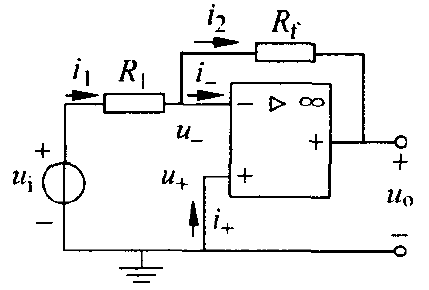
\includegraphics[height=100pt]{assets/3/反向比例放大器.png}
    \caption{\bfseries 同相比例放大器}
\end{subfigure}\begin{subfigure}[t]{0.4\textwidth}\centering
    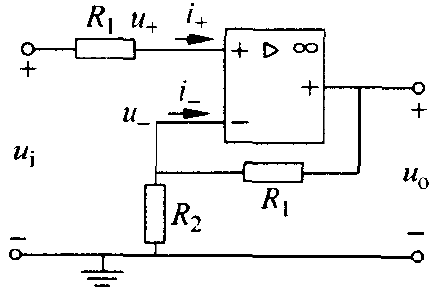
\includegraphics[height=100pt]{assets/3/同相比例放大器.png}
    \caption{\bfseries 反向比例放大器}
\end{subfigure}
\caption{\bfseries 比例放大器}
\end{figure}

\section{第一次仿真作业 (仿真 2-1)}

\subsection{单 OPA 实现电压运算}

电路如图 \ref{单 OPA 实现 电压运算} (a) 所示,接线端示意图见图 \ref{单 OPA 实现 电压运算} (b)。

\begin{figure}[H]\centering
\begin{subfigure}[t]{0.43\textwidth}\centering
    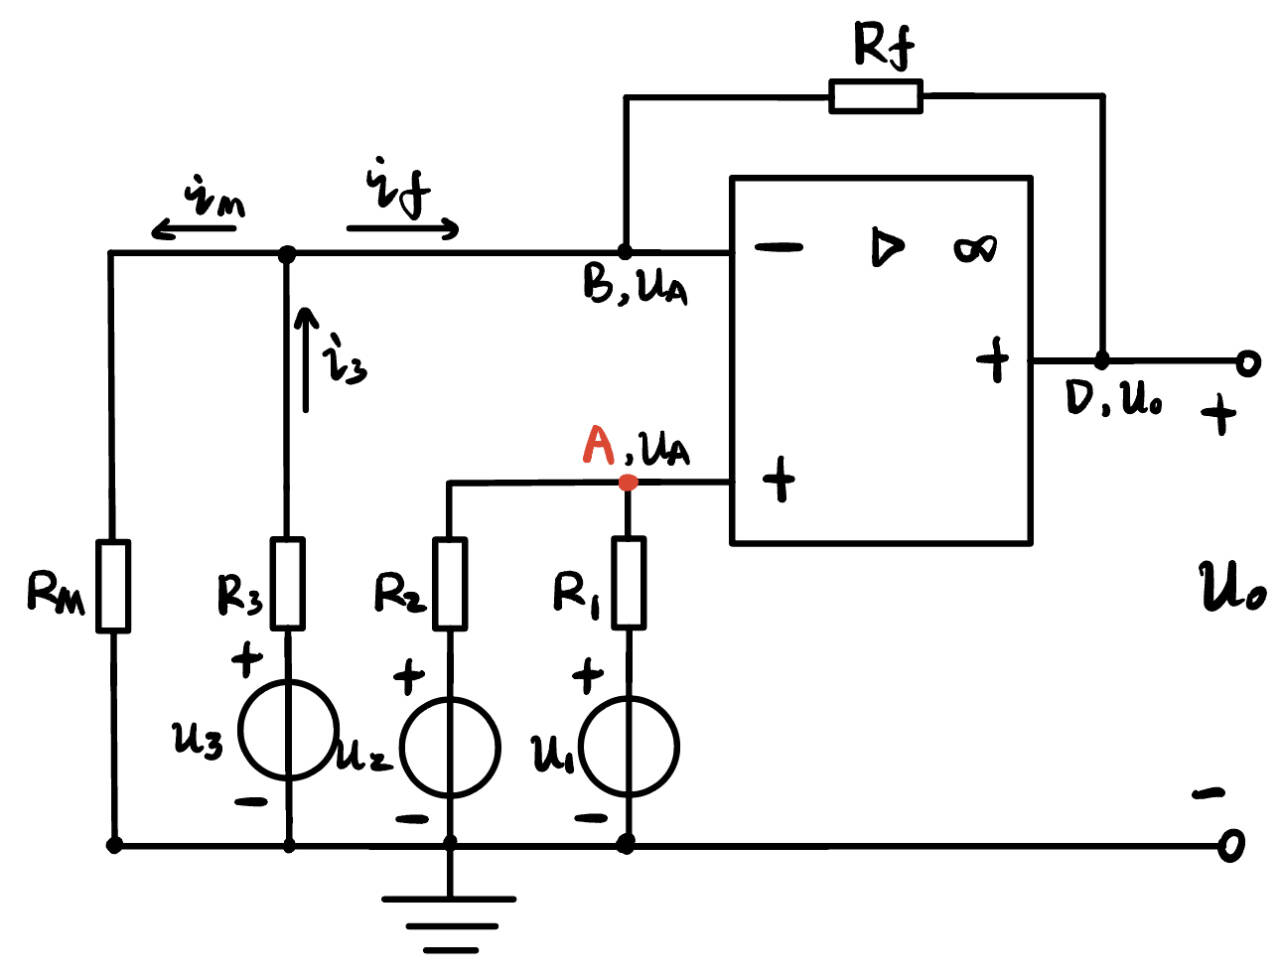
\includegraphics[height=150pt]{assets/3/单OPA.png}
    \caption{\bfseries 电路示意图 }
\end{subfigure}\begin{subfigure}[t]{0.43\textwidth}\centering
    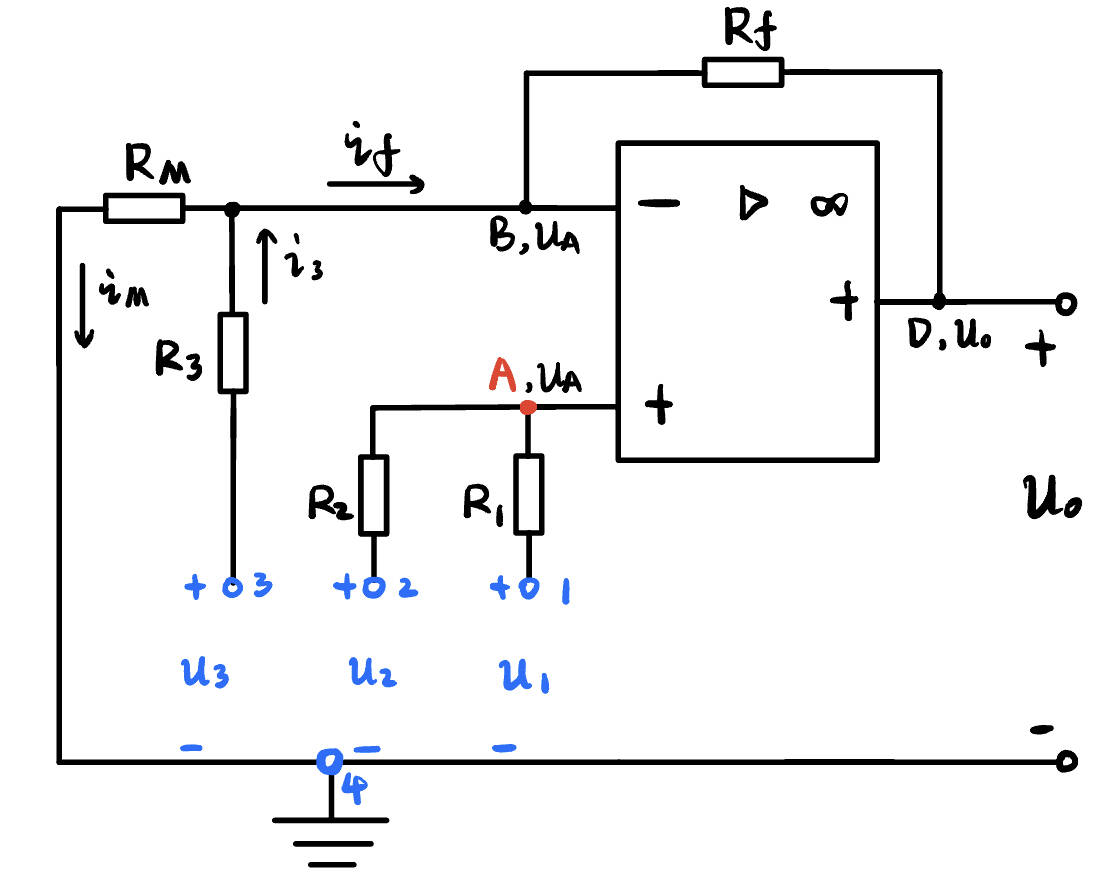
\includegraphics[height=150pt]{assets/3/单OPA接线端.png}
    \caption{\bfseries 接线端示意图 }
\end{subfigure}
\caption{\bfseries 单 OPA 实现 电压运算 }\label{单 OPA 实现 电压运算}
\end{figure}

下面分析其输出特性。由虚断,在 $u_1$ 和 $u_2$ 构成的回路中,设正向流经 $u_2$ 的电流为 $i_2$,则有:
\begin{equation}
i_2 = \frac{u_2 - u_1}{R_1+R_2}
\Longrightarrow  
u_A = u_2 - i_2R_2 = \frac{R_2u_1 + R_1u_2}{R_1 + R_2}
\end{equation}
由虚短,B 点的电势也为 $u_A$,于是:
\begin{equation}
i_3 = \frac{u_3 - u_A}{R_3},\ i_M = \frac{u_A}{R_M} \Longrightarrow  i_f = i_3 - i_M = \frac{u_3 - u_A}{R_3} - \frac{u_A}{R_M} = \frac{u_3}{R_3} - (\frac{1}{R_3} + \frac{1}{R_M})u_A
\end{equation}
由虚断和 KVL:
\begin{equation}
u_o = u_A - i_fR_f = u_A - \frac{R_f}{R_3}u_3 + (\frac{R_f}{R_3} + \frac{R_f}{R_M})u_A = \left( 1 +  \frac{R_f}{R_3} + \frac{R_f}{R_M}\right)u_A - \frac{R_f}{R_3}u_3
\end{equation}
将 $u_A$ 的表达式代入,最终得到:
\begin{equation}
\boxed{
    u_o = \left( 1 +  \frac{R_f}{R_3} + \frac{R_f}{R_M}\right)\frac{1}{\frac{R_1}{R_2} + 1}u_1 
    + \left( 1 +  \frac{R_f}{R_3} + \frac{R_f}{R_M}\right)\frac{\frac{R_1}{R_2}}{\frac{R_1}{R_2} + 1}u_2
    - \frac{R_f}{R_3}u_3
}
\end{equation}
我们需要 $u_1,u_2,u_3$ 前的系数分别为 3, 2, -0.5,于是有:
\begin{equation}
\begin{cases}
    \left( 1 +  \frac{R_f}{R_3} + \frac{R_f}{R_M}\right)\frac{1}{\frac{R_1}{R_2} + 1} = 3 \vspace*{5pt}\\ 
    \vspace*{5pt}
    \left( 1 +  \frac{R_f}{R_3} + \frac{R_f}{R_M}\right)\frac{\frac{R_1}{R_2}}{\frac{R_1}{R_2} + 1} = 2 \\ 
    -\frac{R_f}{R_3} = -0.5
\end{cases}
\Longrightarrow 
\begin{cases}
    R_1 = \frac{2}{3}R_2 &,\ R_2 > 0\\ 
    R_3 = 2R_f,\ R_M = \frac{2}{7}R_f &,\ R_f >0\\
\end{cases}
\end{equation}
为了保持 OPA 的理想性,我们应选择 $\KO$ 量级的电阻,同时,为了降低电路的整体功率,减少消耗,电阻阻值应该尽量大。综合下来,不妨选取 $R_2 = 6 \KO,\ R_f = 3.5 \KO$,此时所有电阻阻值为:
\begin{equation}
R_1 = 4\KO,\ R_2 = 6\KO,\ R_3 = 7\KO,\ R_M = 1\KO,\ R_f = 3.5\KO
\end{equation}

如图,在 Multisim 中进行仿真,得到的结果如下表所示:

% \usepackage[longtable]{multirow}
% \usepackage{longtable}


\begin{longtable}{|c|c|c|c|c|c|c|c|c|c|c|c|c|} 
    \hline
    \multirow{3}{*}{项目} & \multicolumn{3}{c|}{1} & \multicolumn{3}{c|}{2} & \multicolumn{3}{c|}{3} & \multicolumn{3}{c|}{4}  \\* 
    \cline{2-13}
                      & $x,\ u_1$ & $y,\ u_2$ & $z,\ u_3$  & $x,\ u_1$ & $y,\ u_2$ & $z,\ u_3$               &  $x,\ u_1$ & $y,\ u_2$ & $z,\ u_3$             &  $x,\ u_1$ & $y,\ u_2$ & $z,\ u_3$              \\* 
    \cline{2-13}
                      & 1     & 1     & 1      & 1 & 3 & 2              & -2 & 2 & 0             & 3 & 3 & 2               \endfirsthead 
    \hline
    理论输出 $(\mathrm{V})$             & \multicolumn{3}{c|}{$3+2-0.5 = 4.5$}  & \multicolumn{3}{c|}{$3+6-1=8$}  & \multicolumn{3}{c|}{$-6+4-0 = -2$}  & \multicolumn{3}{c|}{$9+6-1=14$}   \\ 
    \hline
    仿真输出 $(\mathrm{V})$     & \multicolumn{3}{c|}{4.50}  & \multicolumn{3}{c|}{8.00}  & \multicolumn{3}{c|}{-2.00}  & \multicolumn{3}{c|}{10.494}   \\
    \hline
\end{longtable}
由表可见,除了最后一组数据,仿真结果与理论结果完全一致。最后一组之所以不同,是因为输出电压 $u_o$ 超出了此 OPA 的饱和电压 $U_{\text{sat}}$,导致输出电压 $u_o = U_{\text{sat}} = 10.494 \mathrm{V}$。如图所示,此 OPA (LM324ADTBR2G) 的饱和电压为 $10.525 \mathrm{V}$,与解释相符。

\subsection{一些失败的例子}
注意到,减法器是在反相加法器的基础上,串联入电压源(和电阻)改变了 $u_+$ 端的电压。这样,在最终的输出电压 $u_o$ 中,$u_-$ 端的电源电压会带负号,$u_+$ 端的电源电压带正号。用类似的思想,我们可以对减法器进行改造,最终仅用一个 OPA 便实现 $3x+2y-0.5z$ 的电压运算。

一种方法是向 $u_+$ 端再串联一个电压源,使得输出 $u_o$ 中两正一负,然后通过电阻值来调整系数,但是,这样不满足接线端的要求(三正一共地)。另一种方法是向 $u_-$ 端再并联一个电压源,使得输出 $u_o$ 中两负一正($-u_1,\ -u_2,\ +u_3$),最后通过电阻值来调整系数,但是,这样得到的是两负一正而不是两正一负,虽满足了接线端要求,却不是我们需要的结果。

其实,我们只需要向 $u_+$ 端的电压源(包括电阻)再并联一个电压源(包括)电阻即可,如图所示。下面分析其输出特性。

\begin{figure}[H]\centering
\begin{subfigure}[t]{0.48\textwidth}\centering
    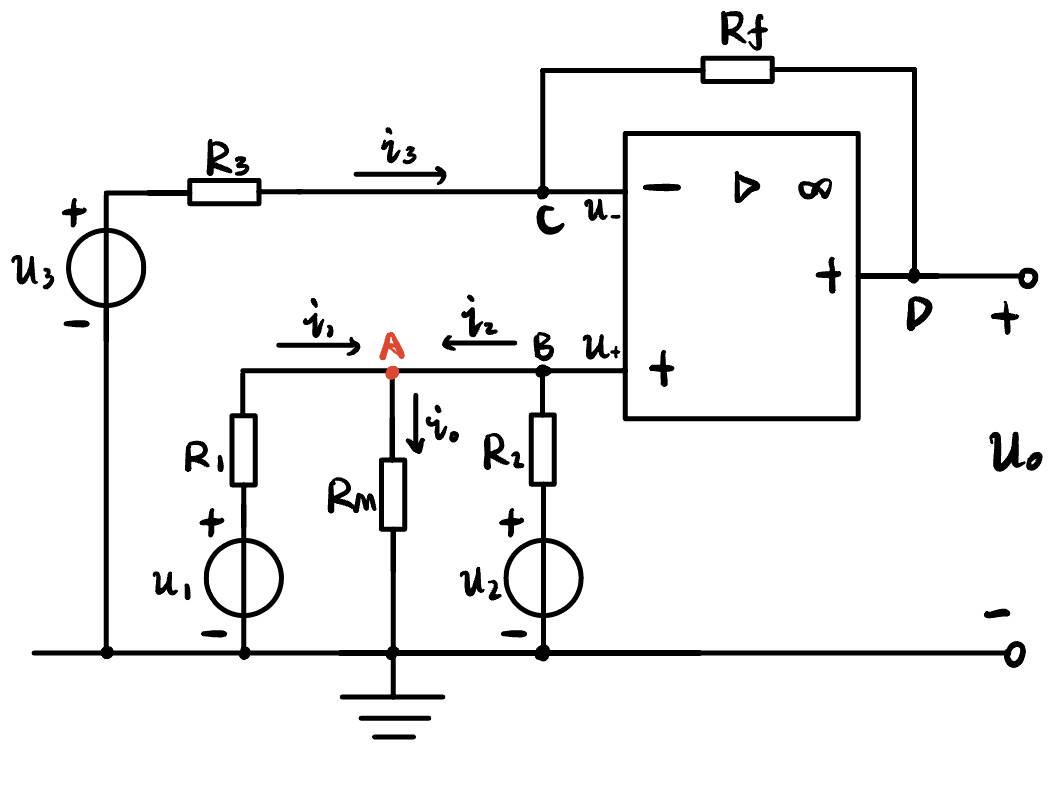
\includegraphics[height=150pt]{assets/3/失败的例子.png}
    \caption{\bfseries 失败的例子 }
\end{subfigure}\begin{subfigure}[t]{0.45\textwidth}\centering
    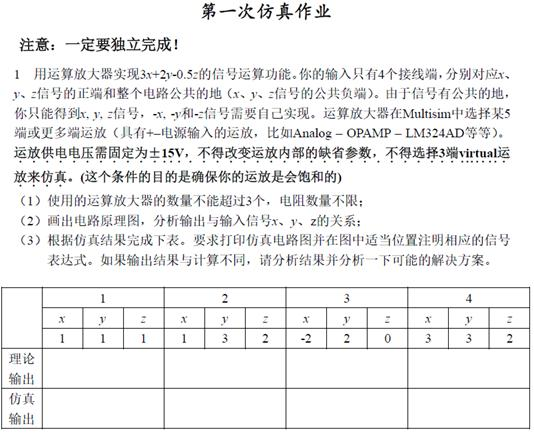
\includegraphics[height=150pt]{assets/3/image (5).jpg}
    \caption{\bfseries 仿真作业 2-1 }
\end{subfigure}
\caption{\bfseries 示意图 }
\end{figure}

在 $u_1, R_1, u_2, R_2 $ 和 $R_M$ 构成的局部电路中,由 KVC:
\begin{gather}
\begin{cases}
    u_1 - R_1i_1 - R_M(i_1 + i_2) = 0 \\
u_2 - R_2i_2 - R_M(i_1 + i_2) = 0
\end{cases}
\Longrightarrow 
\begin{cases}
    i_1 = \frac{(R_2+R_M)u_1 - R_Mu_2}{R_1R_2 +R_1R_M + R_2R_M} \\ 
    i_2 = \frac{(R_1+R_M)u_2 - R_Mu_1}{R_1R_2 +R_1R_M + R_2R_M} \\ 
\end{cases}
\end{gather}
由此得点 A 处的电势 $u_A$:
\begin{equation}
    u_A = \frac{R_2R_Mu_1 + R_1R_Mu_2}{R_1R_2 +R_1R_M + R_2R_M}
\end{equation}
也即点 B 和非反相输入端的电势 $u_+ = u_B = u_A$。由虚短,$u_- = u_+$,可得电流 $i_3$:
\begin{equation}
i_3 = \frac{u_3 - u_-}{R_3} = \frac{1}{R_3}(u_3 - \frac{R_2R_Mu_1 + R_1R_Mu_2}{R_1R_2 +R_1R_M + R_2R_M}) 
\end{equation}
由虚断,经过电阻 $R_f$ 求得 D 点电势,也即输出电压 $u_o$:
\begin{align}
u_o &= u_A - i_3R_f = (1+\frac{R_f}{R_3})u_A - \frac{R_f}{R_3}u_3 
\\
&= (1+\frac{R_f}{R_3})\cdot \frac{\frac{R_M}{R_1}u_1 + \frac{R_M}{R_2}u_2}{1 + \frac{R_M}{R_1} + \frac{R_M}{R_2}} - \frac{R_f}{R_3}u_3
\\ 
&=\frac{1+\frac{R_f}{R_3}}{1 + \frac{R_M}{R_1} + \frac{R_M}{R_2}}
\left( \frac{R_M}{R_1}u_1 + \frac{R_M}{R_2}u_2  \right) - \frac{R_f}{R_3}u_3
\end{align}

最后调整电阻阻值。为了保持 OPA 的理想性,电阻需要在 $\KO$ 量级,令电阻比例如下:
\begin{equation}
\begin{cases}
    \frac{R_f}{R_3} = 0.5 \\ 
    \frac{1+\frac{R_f}{R_3}}{1 + \frac{R_M}{R_1} + \frac{R_M}{R_2}}\cdot \frac{R_M}{R_1} = 3 \\ 
    \frac{1+\frac{R_f}{R_3}}{1 + \frac{R_M}{R_1} + \frac{R_M}{R_2}}\cdot \frac{R_M}{R_2} = 2
\end{cases}\Longrightarrow 
\begin{cases}
    R_f = \frac{1}{2}R_3 \\ 
    R_1 =  -2R_M\\ 
    R_2 = -\frac{4}{3}R_M
\end{cases}
\end{equation}
显然,这不可能实现,舍弃。









\section{第一次仿真作业 (2)}

在负电阻中,OPA 输出电压 $u_o$:
\begin{equation}
u_o = \left(1 + \frac{R_2}{R}\right)u_i
\end{equation}
我们选择的 OPA 饱和电压 $U_{\text{sat}} = 1.5\ V$,因此,当 $u_i < $ 或 $u_i >$ 时,OPA 工作在饱和区,此时 $u_o = \pm U_{\text{sat}}$ 为定值,且虚短不再成立,电流 $i_1$:
\begin{equation}
i_1 = \frac{u_1 - u_o}{R_1} = 
\begin{cases}
    \frac{u_1 - U_{\text{sat}}}{R_1} &, u_1 > \\ 
    \frac{u_1 + U_{\text{sat}}}{R_1} &, u_1 < \\ 
\end{cases}
\end{equation}

\begin{figure}[H]\centering
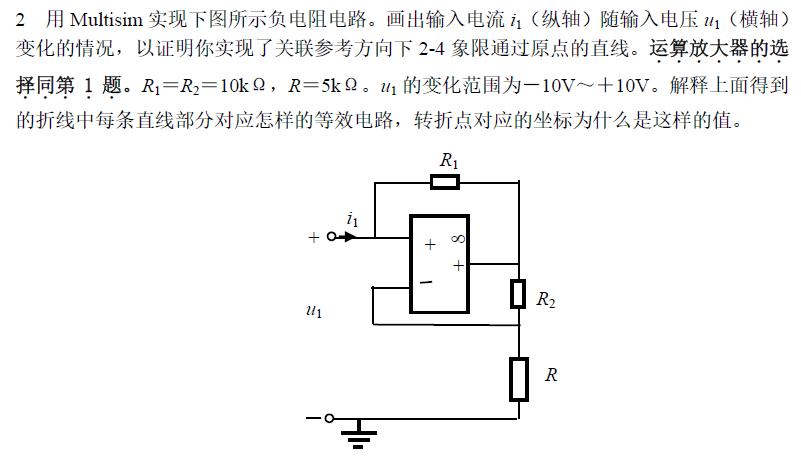
\includegraphics[width=0.45\textwidth]{assets/3/ee57b549a02999b0856af303ac0e8510.jpg}
\caption{\bfseries 第一次仿真作业 (2)}\label{第一次仿真作业 (2)}
\end{figure}

\chapter{2024.9.17 - 2024.9.23}\thispagestyle{fancy}

\section{习题集 }
\section{习题集 }
\section{习题集 }
\section{习题集 }
\section{习题集 }
\section{习题集 }
\section{习题集 }

\chapter{2024.9.24 - 2024.9.30}\thispagestyle{fancy}

\section{习题集 }
\section{习题集 }
\section{习题集 }
\section{习题集 }
\section{习题集 }
\section{习题集 }
\section{习题集 }

\chapter{2024.10.1 - 2024.10.7}\thispagestyle{fancy}

\section{习题集 }
\section{习题集 }
\section{习题集 }
\section{习题集 }
\section{习题集 }
\section{习题集 }
\section{习题集 }

\chapter{2024.10.8 - 2024.10.14}\thispagestyle{fancy}

\section{习题集 }
\section{习题集 }
\section{习题集 }
\section{习题集 }
\section{习题集 }
\section{习题集 }
\section{习题集 }

\chapter{2024.10.15 - 2024.10.21}\thispagestyle{fancy}

\section{习题集 }
\section{习题集 }
\section{习题集 }
\section{习题集 }
\section{习题集 }
\section{习题集 }
\section{习题集 }

\chapter{2024.10.22 - 2024.10.28}\thispagestyle{fancy}

\section{习题集 }
\section{习题集 }
\section{习题集 }
\section{习题集 }
\section{习题集 }
\section{习题集 }
\section{习题集 }


























































































































\end{document}



% VScode 常用快捷键:

% F2:                       变量重命名
% Ctrl + Enter:             行中换行
% Alt + up/down:            上下移行
% 鼠标中键 + 移动:           快速多光标
% Shift + Alt + up/down:    上下复制
% Ctrl + left/right:        左右跳单词
% Ctrl + Backspace/Delete:  左右删单词    
% Shift + Delete:           删除此行
% Ctrl + J:                 打开 VScode 下栏(输出栏)
% Ctrl + B:                 打开 VScode 左栏(目录栏)
% Ctrl + `:                 打开 VScode 终端栏
% Ctrl + 0:                 定位文件
% Ctrl + Tab:               切换已打开的文件(切标签)
% Ctrl + Shift + P:         打开全局命令(设置)

% Latex 常用快捷键

% Ctrl + Alt + J:           由代码定位到PDF
% 


% Git提交规范:
% update: Linear Algebra 2 notes
% add: Linear Algebra 2 notes
% import: Linear Algebra 2 notes
% delete: Linear Algebra 2 notes














































































































































































































































































































































































































































































































































































































\end{document}

% VScode 常用快捷键:

% F2:                       变量重命名
% Ctrl + Enter:             行中换行
% Alt + up/down:            上下移行
% 鼠标中键 + 移动:           快速多光标
% Shift + Alt + up/down:    上下复制
% Ctrl + left/right:        左右跳单词
% Ctrl + Backspace/Delete:  左右删单词    
% Shift + Delete:           删除此行
% Ctrl + J:                 打开 VScode 下栏(输出栏)
% Ctrl + B:                 打开 VScode 左栏(目录栏)
% Ctrl + `:                 打开 VScode 终端栏
% Ctrl + 0:                 定位文件
% Ctrl + Tab:               切换已打开的文件(切标签)
% Ctrl + Shift + P:         打开全局命令(设置)

% Latex 常用快捷键

% Ctrl + Alt + J:           由代码定位到PDF
% 


% Git提交规范:
% update: Linear Algebra 2 notes
% add: Linear Algebra 2 notes
% import: Linear Algebra 2 notes
% delete: Linear Algebra 2 notes
